%%%%%%%%%%%%%%%%%%%%%%%%%%%%%%%%%%%%%%%%%
% Beamer Presentation
% LaTeX Template
% Version 1.0 (10/11/12)
%
% This template has been downloaded from:
% http://www.LaTeXTemplates.com
%
% License:
% CC BY-NC-SA 3.0 (http://creativecommons.org/licenses/by-nc-sa/3.0/)
%
%%%%%%%%%%%%%%%%%%%%%%%%%%%%%%%%%%%%%%%%%

%----------------------------------------------------------------------------------------
%	PACKAGES AND THEMES
%----------------------------------------------------------------------------------------

\documentclass{beamer}

\mode<presentation> {

% The Beamer class comes with a number of default slide themes
% which change the colors and layouts of slides. Below this is a list
% of all the themes, uncomment each in turn to see what they look like.

%\usetheme{default}
%\usetheme{AnnArbor}
%\usetheme{Antibes}
%\usetheme{Bergen}
%\usetheme{Berkeley}
%\usetheme{Berlin}
%\usetheme{Boadilla}
%\usetheme{CambridgeUS}
%\usetheme{Copenhagen}
%\usetheme{Darmstadt}
%\usetheme{Dresden}
%\usetheme{Frankfurt}
%\usetheme{Goettingen}
%\usetheme{Hannover}
%\usetheme{Ilmenau}
%\usetheme{JuanLesPins}
%\usetheme{Luebeck}
\usetheme{Madrid}
%\usetheme{Malmoe}
%\usetheme{Marburg}
%\usetheme{Montpellier}
%\usetheme{PaloAlto}
%\usetheme{Pittsburgh}
%\usetheme{Rochester}
%\usetheme{Singapore}
%\usetheme{Szeged}
%\usetheme{Warsaw}

% As well as themes, the Beamer class has a number of color themes
% for any slide theme. Uncomment each of these in turn to see how it
% changes the colors of your current slide theme.

%\usecolortheme{albatross}
\usecolortheme{beaver}
%\usecolortheme{beetle}
%\usecolortheme{crane}
%\usecolortheme{dolphin}
%\usecolortheme{dove}
%\usecolortheme{fly}
%\usecolortheme{lily}
%\usecolortheme{orchid}
%\usecolortheme{rose}
%\usecolortheme{seagull}
%\usecolortheme{seahorse}
%\usecolortheme{whale}
%\usecolortheme{wolverine}

%\setbeamertemplate{footline} % To remove the footer line in all slides uncomment this line
%\setbeamertemplate{footline}[page number] % To replace the footer line in all slides with a simple slide count uncomment this line

%\setbeamertemplate{navigation symbols}{} % To remove the navigation symbols from the bottom of all slides uncomment this line

\setbeamertemplate{frametitle}[default][center]
}

\usepackage{graphicx} % Allows including images
\usepackage{booktabs} % Allows the use of \toprule, \midrule and \bottomrule in tables
\usepackage{multimedia}
%\usepackage{movie15}
\usepackage{caption}
\usepackage{subcaption}
\usepackage{amsfonts}
\usepackage{epstopdf}
\usepackage{bigints}
\usepackage{amsmath}
\usepackage{hyperref}
\usepackage{verbatim}
\usepackage{mathrsfs}
\usepackage{color}
\usepackage[outline]{contour}
\usepackage{multirow}

\contourlength{1pt}

\newcommand\Bo{\mbox{\textit{Bo}}}  % Bond number
\newcommand\Rey{\mbox{\textit{Re}}}  % Reynolds number
\newcommand\Ri{\mbox{\textit{Ri}}}  % Richardson number

\def\Xint#1{\mathchoice
{\XXint\displaystyle\textstyle{#1}}%
{\XXint\textstyle\scriptstyle{#1}}%
{\XXint\scriptstyle\scriptscriptstyle{#1}}%
{\XXint\scriptscriptstyle\scriptscriptstyle{#1}}%
\!\int}
\def\XXint#1#2#3{{\setbox0=\hbox{$#1{#2#3}{\int}$}
\vcenter{\hbox{$#2#3$}}\kern-.5\wd0}}
\def\ddashint{\Xint=}
\def\dashint{\Xint-}

%----------------------------------------------------------------------------------------
%	TITLE PAGE
%----------------------------------------------------------------------------------------

\title[Modeling volcanic processes]{Gravity currents in volcanology} % The short title appears at the bottom of every slide, the full title is only on the title page

\author[Paul Jarvis]{Paul A. Jarvis} % Your name
\institute[UNIGE] % Your institution as it will appear on the bottom of every slide, may be shorthand to save space
{
\textit{paul.jarvis@unige.ch} % Your email address
}
\date{22nd November 2019} % Date, can be changed to a custom date
\begin{columns}

  \begin{column}{0.33\paperwidth}
    $$
\includegraphics[width=0.3\paperwidth]{UNIGE_logo.jpg}$$
  \end{column}

  \begin{column}{0.33\paperwidth}
    $$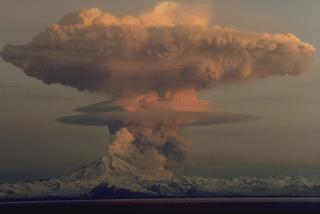
\includegraphics[width=0.3\paperwidth]{redoubt.jpg}$$
  \end{column}

  \begin{column}{0.33\paperwidth}
    $$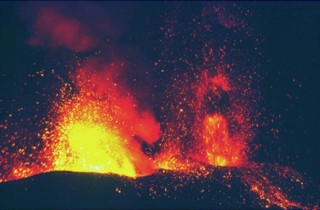
\includegraphics[width=0.3\paperwidth]{etna.jpg}$$
  \end{column}
  
\end{columns}
\vspace{-2cm}

\DeclareMathOperator\erf{erf}

\begin{document}

\begin{frame}
\titlepage % Print the title page as the first slide
\end{frame}

%\begin{frame}
%\frametitle{Overview} % Table of contents slide, comment this block out to remove it
%\tableofcontents % Throughout your presentation, if you choose to use \section{} and \subsection{} commands, these will automatically be printed on this slide as an overview of your presentation
%\end{frame}


%----------------------------------------------------------------------------------------
%	PRESENTATION SLIDES
%----------------------------------------------------------------------------------------

%------------------------------------------------
%\section{First Section} % Sections can be created in order to organize your presentation into discrete blocks, all sections and subsections are automatically printed in the table of contents as an overview of the talk
%------------------------------------------------

%\subsection{Subsection Example} % A subsection can be created just before a set of slides with a common theme to further break down your presentation into chunks

\begin{frame}
  \frametitle{Lava flows - Flow on a slope}

  Consider flow of a viscous fluid on a slope \\

  \begin{columns}[t]

    \begin{column}{0.5\paperwidth}

      $$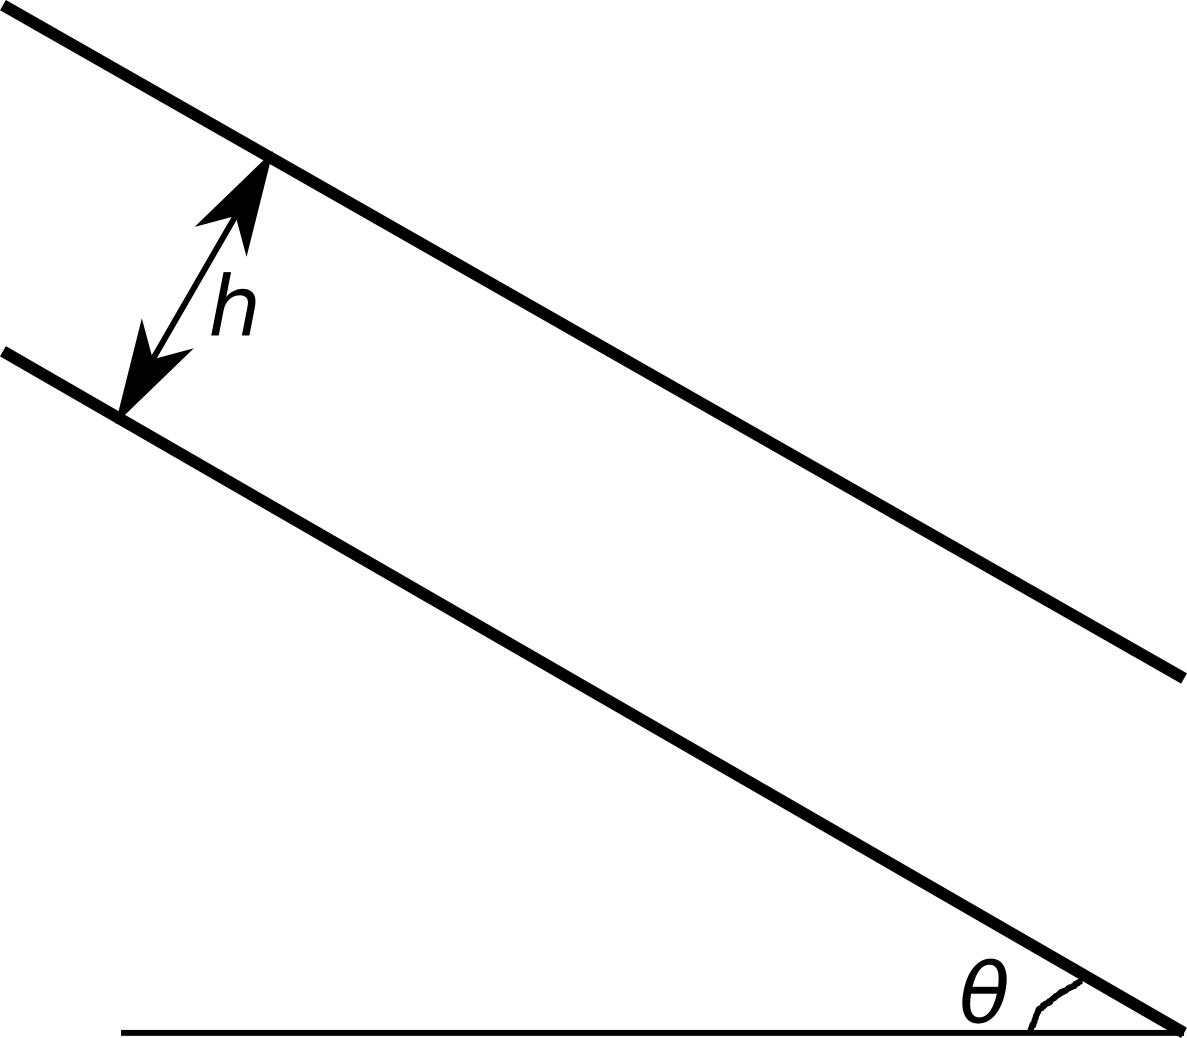
\includegraphics[width=0.3\paperwidth]{slope_flow.png}$$

    \end{column}

    \begin{column}{0.5\paperwidth}

      Want to determine shear stress at base of flow \\

      \vspace{1cm}
      
      \textbf{Shear stress} = Force per unit area extered on ground \\
    \end{column}
    
  \end{columns}
  
\end{frame}
%-----------------------------------------------
\begin{frame}
  \frametitle{Lava flows - Flow on a slope}

  \begin{columns}[t]

    \begin{column}{0.5\paperwidth}

      $$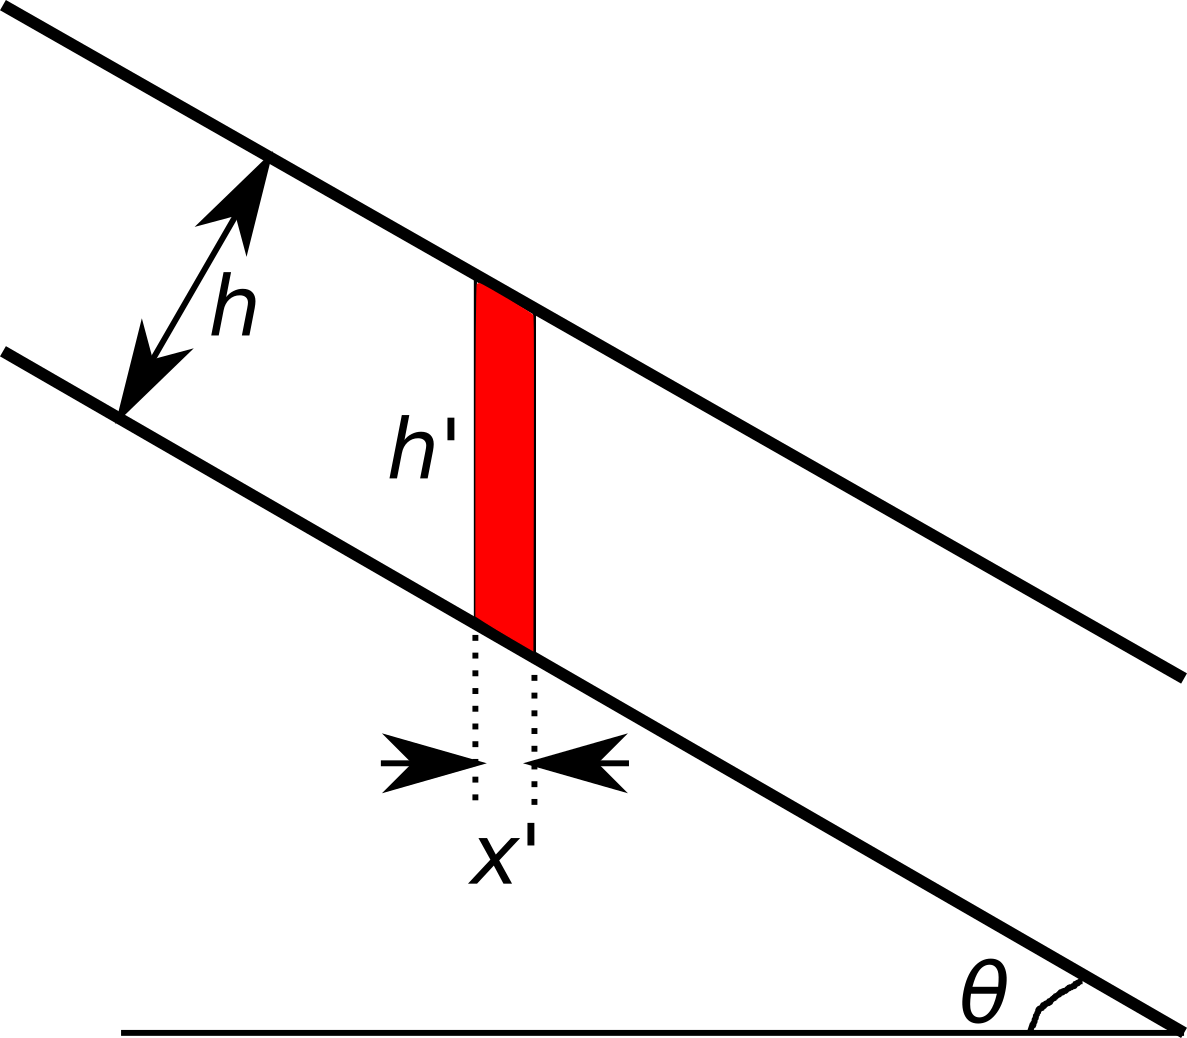
\includegraphics[width=0.3\paperwidth]{slope_flow_vol.png}$$

      $$ h' = \frac{h}{\cos\theta} $$

      $$ W = \frac{\rho h x' d g}{\cos \theta}$$
    \end{column}

    \begin{column}{0.5\paperwidth}

      Consider a volume of a thin slice

      $$ V = h' x' d $$

      where $d$ = width of flow \\

      So, total weight of column:

      $$ W = \rho V g = \rho h' x' d g $$

      \vspace{-0.5cm}
      $$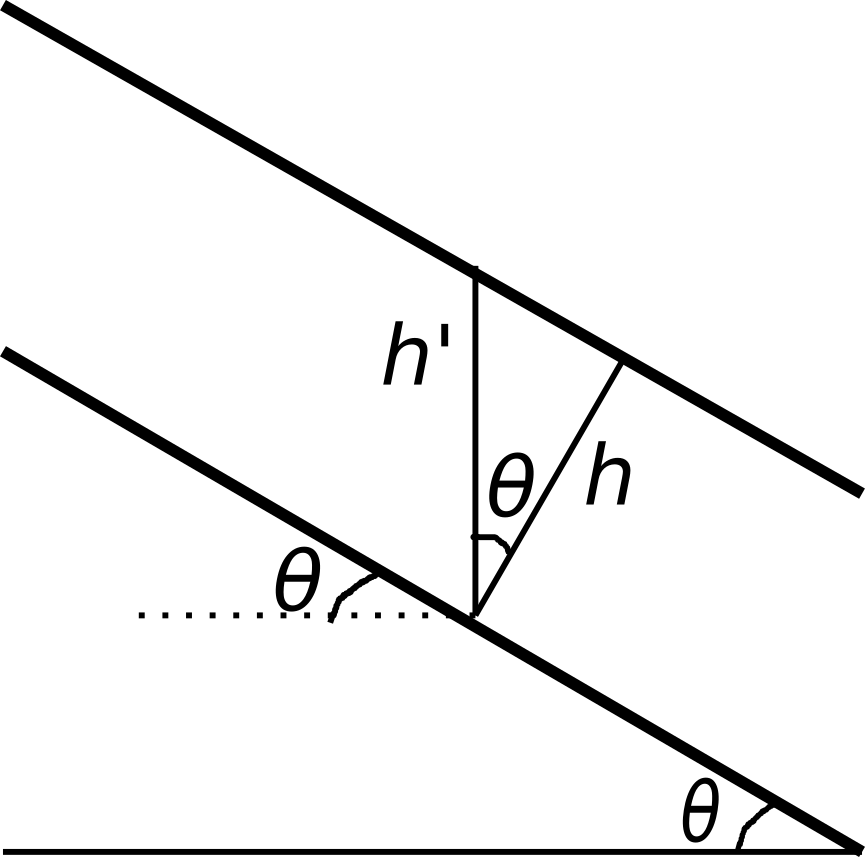
\includegraphics[width=0.3\paperwidth]{slope_trig.png}$$
    \end{column}
    
  \end{columns}
  
\end{frame}
%-----------------------------------------------
\begin{frame}
  \frametitle{Lava flows - Flow on a slope}

  \begin{columns}[t]

    \begin{column}{0.5\paperwidth}

      $$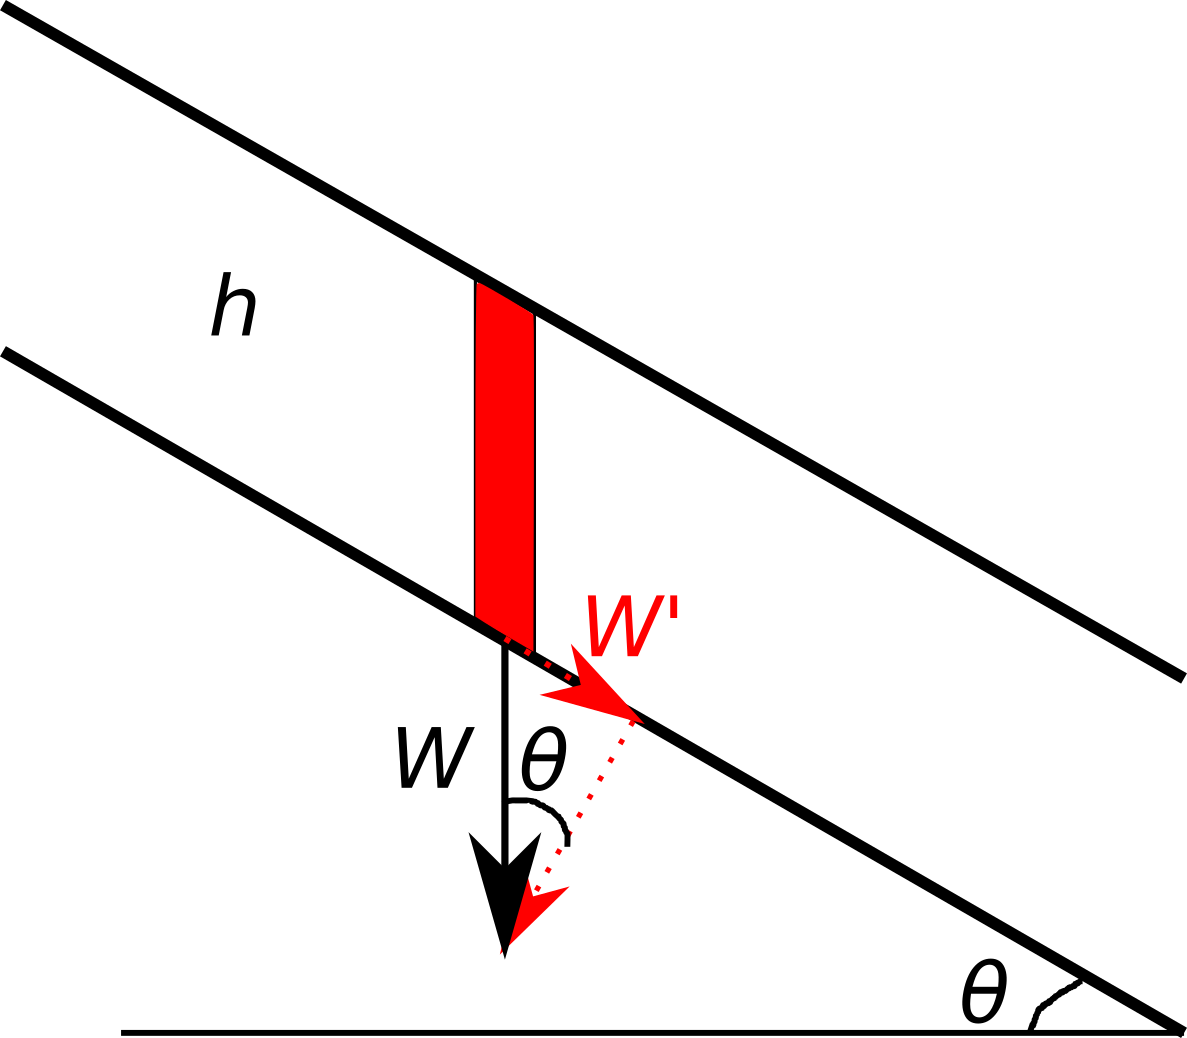
\includegraphics[width=0.3\paperwidth]{slope_flow_weight.png}$$

      Area under column $A = X d = \frac{x' d}{\cos \theta}$

      Shear stress:

      $$ \tau = \frac{W'}{A} = \rho g h \sin \theta $$
    \end{column}

    \begin{column}{0.5\paperwidth}

      Downslope component of weight:

      $$ W' = W \sin \theta $$

      $$ W' = \frac{\rho h x' d g \sin \theta}{\cos \theta}$$

      $$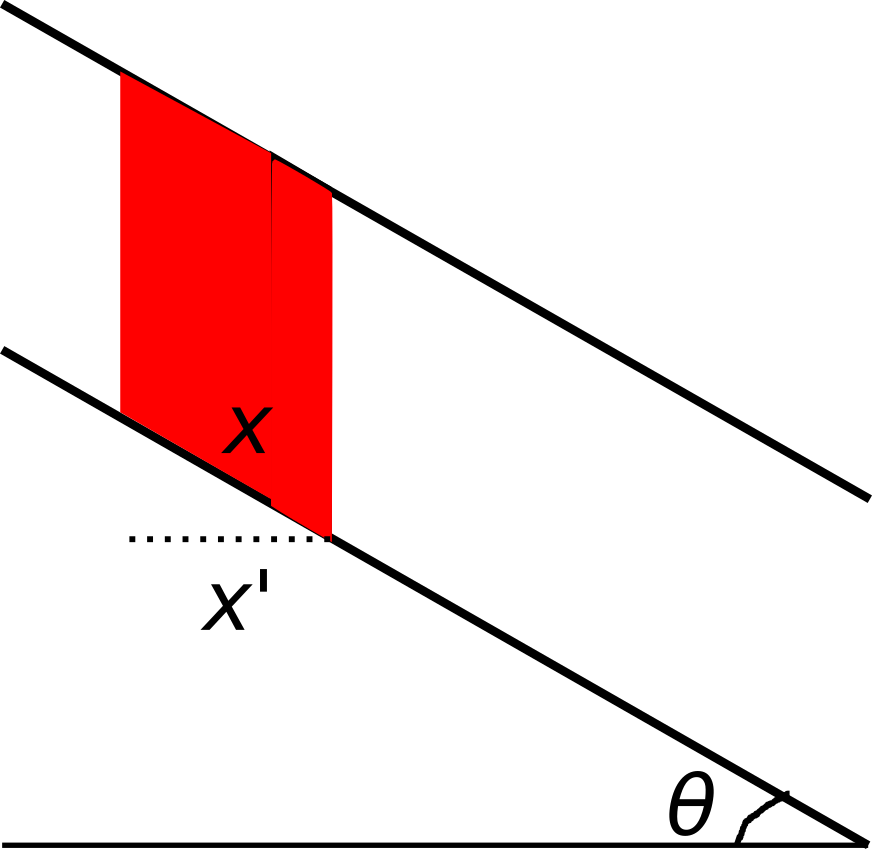
\includegraphics[width=0.3\paperwidth]{slope_flow_area.png}$$
      
    \end{column}
    
  \end{columns}
  
\end{frame}
%-----------------------------------------------
\begin{frame}
  \frametitle{Lava flow rheology}

  \begin{columns}[t]

    \begin{column}{0.5\paperwidth}

      $$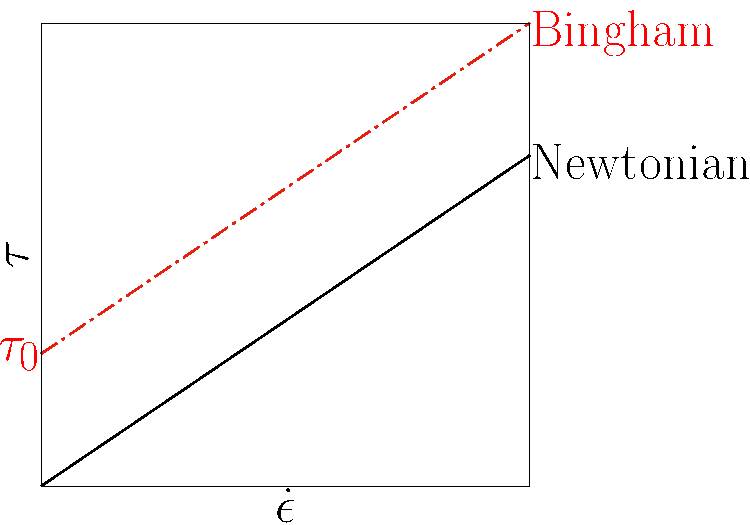
\includegraphics[width=\textwidth]{flow_curves.pdf}$$

    \end{column}

    \begin{column}{0.5\paperwidth}

      Crystal-free lavas behave as Newtonian fluids \\

      \vspace{1cm}

      Partially crystallised lavas have a yield stress $\tau_{0}$ \\

      \vspace{1cm}

      Lavas have a minimum thickness below which they cannot flow:

      $$ h_{0} = \frac{\tau_{0}}{\rho g \sin \theta}$$

      This thickness depends on the topography \\
    \end{column}
    
  \end{columns}
  
\end{frame}
%-----------------------------------------------
\begin{frame}
  \frametitle{Jeffrey's model for lava flow velocity}

  \begin{columns}[t]

    \begin{column}{0.5\paperwidth}

      $$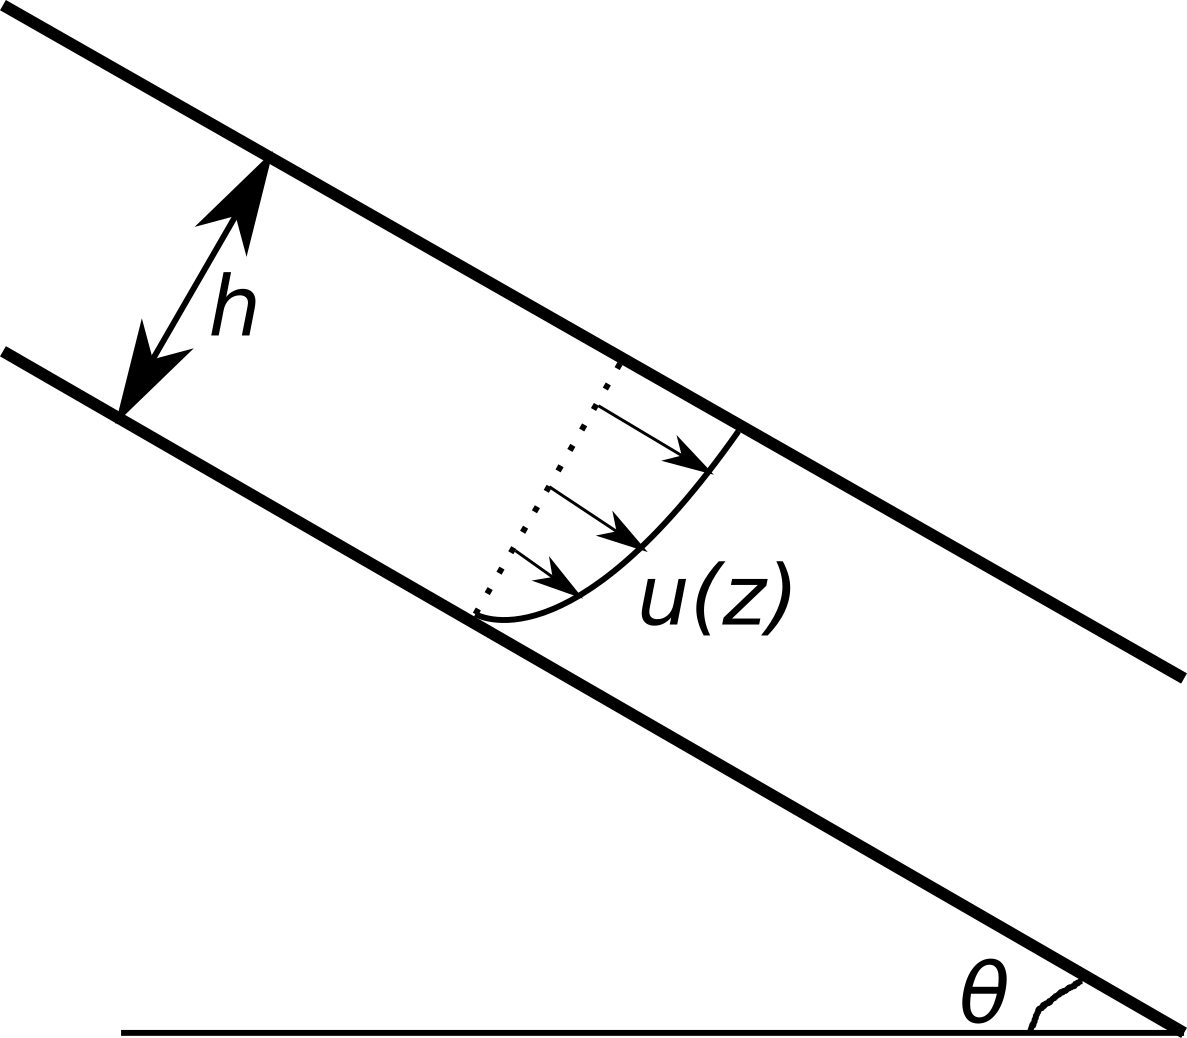
\includegraphics[width=\textwidth]{slope_vel.png}$$

    \end{column}

    \begin{column}{0.5\paperwidth}

      Mean velocity inside a channel:

      $$ \bar{u} = \frac{h^{2} \rho g \sin \theta}{B \eta} $$

      $B$ = constant depending on channel geometry \\

      \vspace{1cm}
      
      Expression is valid for a Newtonian lava \\

      \vspace{1cm}
      
      More complicated models for Bingham fluids \\

    \end{column}
    
  \end{columns}
  
\end{frame}
%-----------------------------------------------
\begin{frame}
  \frametitle{Controls on lava flow}

  Lava flow rates and morphology depend on:

  \begin{columns}[t]

    \begin{column}{0.5\paperwidth}

      \begin{itemize}
      \item Topography \\
        \begin{itemize}
        \item Slope angle \\
        \item Channel geometry (if it exists) \\
        \end{itemize}
      \end{itemize}

    \end{column}

    \begin{column}{0.5\paperwidth}

    \begin{itemize}
    \item Rheology \\
      \begin{itemize}
      \item Viscosity \\
      \item Yield stress \\ 
      \end{itemize}
    \end{itemize}

  \end{column}

\end{columns}

  \vspace{0.5cm}
  
  Rheology is most difficult to assess - it depends on:

  \begin{columns}[t]

    \begin{column}{0.5\paperwidth}

      \begin{itemize}
      \item Composition \\
      \item \textbf{Temperature} \\
      \item Crystallinity \\
      \item Vesivularity \\
      \end{itemize}

    \end{column}

    \begin{column}{0.5\paperwidth}

      \vspace{-1cm}
      
      $$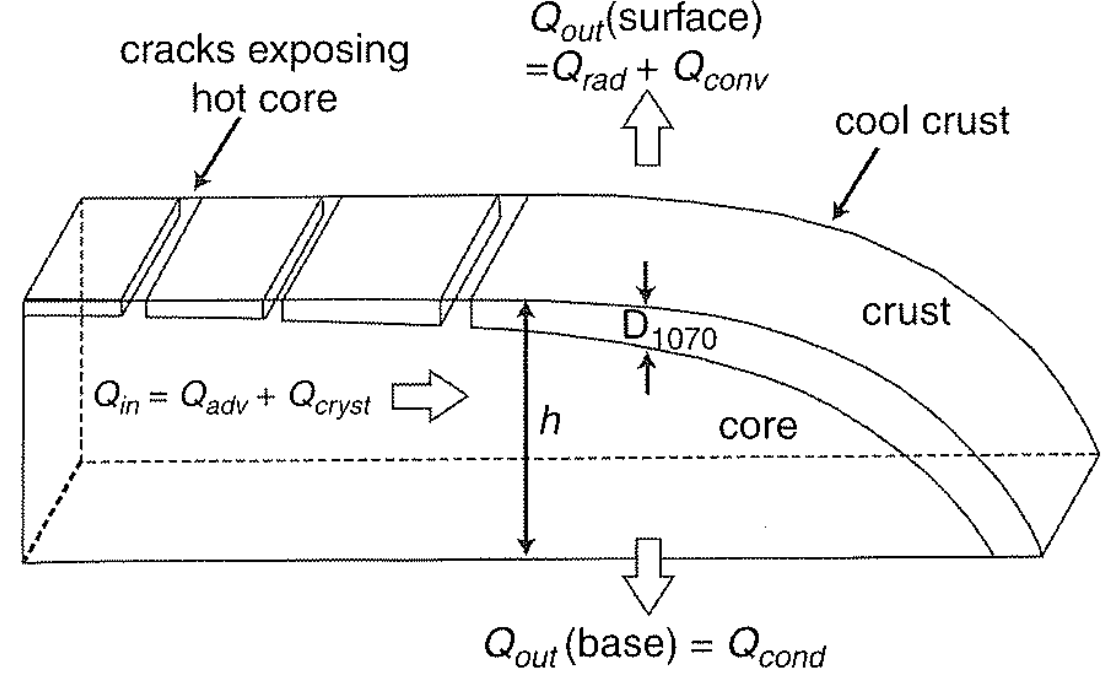
\includegraphics[width=\textwidth]{lava_flow_struct.png}$$
      
    \end{column}

  \end{columns}
  
\end{frame}
%-----------------------------------------------
\begin{frame}
  \frametitle{Heat loss from the flow}

  \begin{columns}[t]

    \begin{column}{0.5\paperwidth}

      \vspace{-1.5cm}
      
      $$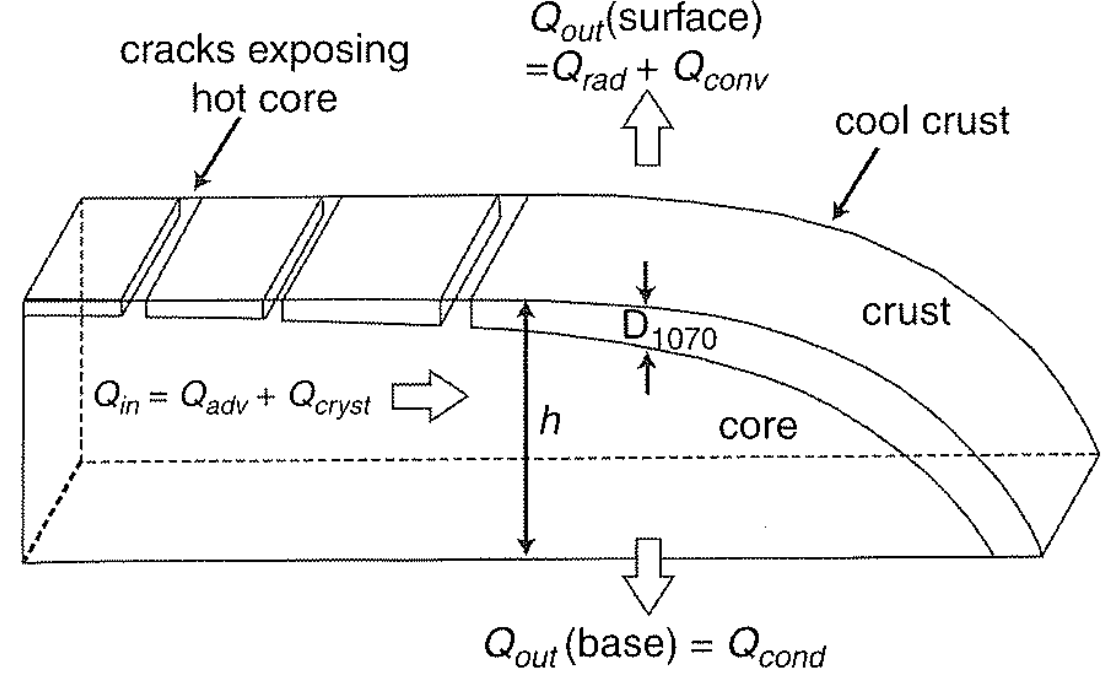
\includegraphics[width=\textwidth]{lava_flow_struct.png}$$

      \vspace{-1cm}

      \begin{itemize}
      \item \textbf{Radiation}
        \begin{itemize}
        \item Emission of heat through EM radiation
        \item Flux determined from Stefan-Boltzman law
          $$ q_{\text{rad}} = \epsilon \sigma(T_{\text{surf}}^{4} - T_{\text{a}}^{4})$$
        \item $\epsilon$ = Emissivity \\
        \item $\sigma$ = Stefan-Boltzmann constant = $5.67 \times 10^{-8}$ W m$^{-2}$ K$^{-4}$  \\
        \end{itemize}
      \end{itemize}
    \end{column}

    \begin{column}{0.5\paperwidth}

      \vspace{-0.5cm}
      
      \begin{itemize}
      \item \textbf{Conduction}
        \begin{itemize}
        \item Direct molecular contact \\
        \item Heat flux (W m$^{-2}$) given by a diffusive term
          $$ q_{\text{cond}} = -k \frac{\mathrm{d} T}{\mathrm{d} x}$$
        \item $k$ = Thermal diffusivity \\
        \end{itemize}
        \vspace{0.9cm}
      \item \textbf{Convection}
        \begin{itemize}
        \item Heat transported through fluid movement
        \item Heat flux given by
          $$ q_{\text{conv}} = h (T_{\text{surf}} - T_{\text{a}}) $$
        \item $h$ = Constant \\
        \end{itemize}
      \end{itemize}
    \end{column}

  \end{columns}
  
\end{frame}
%-----------------------------------------------
\begin{frame}
  \frametitle{`A`$\overline{\text{a}}$}

  \begin{columns}[t]

    \begin{column}{0.48\paperwidth}

      Brecciated surface and basal \textbf{crusts} \\

      \vspace{1cm}

      Coherant \textbf{core} which remains fluid during activity \\

      \vspace{1cm}

      Typically 0.5 - 20 m thick \\

      \vspace{1cm}

      \textbf{Clinkers} - Broken blocks within the crust \\

      \vspace{1cm}

      Forms in lavas of higher viscosity \\


    \end{column}

    \begin{column}{0.48\paperwidth}

      $$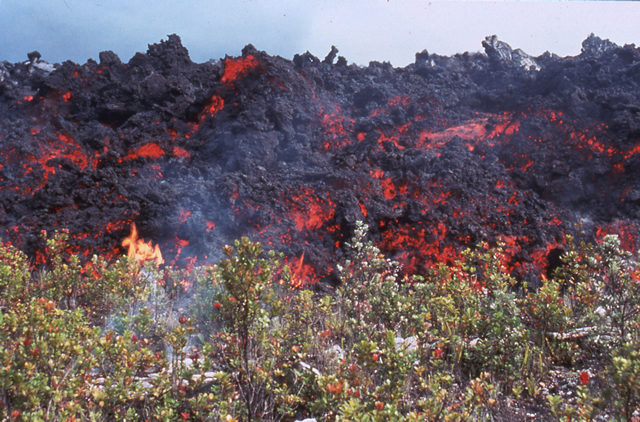
\includegraphics[width=\textwidth]{aa.jpg}$$

    \end{column}

  \end{columns}
  
\end{frame}
%-----------------------------------------------
\begin{frame}
  \frametitle{P$\overline{\text{a}}$hoehoe}

  \begin{columns}[t]

    \begin{column}{0.48\paperwidth}

      Smooth, glassy, coherent surfaces \\

      \vspace{0.3cm}

      Surface folds called \textbf{ropes} \\

      \vspace{0.3cm}

      Individual units have a \textbf{lobate} shape \\

      \vspace{0.3cm}

      Individual flow can consist of 100s-1000s of lobes \\

      \vspace{0.3cm}

      Normally low effusion rates and low viscosity \\

      \vspace{0.3cm}

      Crust is thin but thickens with time \\

      \vspace{0.3cm}

      New lobes \textbf{breakout} through fractures in crust \\

      \vspace{0.3cm}

      Typical thicknesses from 3 - 40 cm \\
      
    \end{column}

    \begin{column}{0.48\paperwidth}

      $$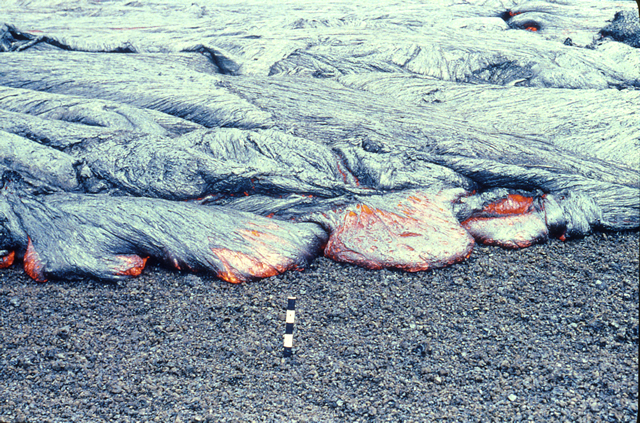
\includegraphics[width=\textwidth]{pahoehoe.jpg}$$

    \end{column}

  \end{columns}
  
\end{frame}
%-----------------------------------------------
\begin{frame}
  \frametitle{Block lavas}

  \begin{columns}[t]

    \begin{column}{0.48\paperwidth}

      Typical of intermediate to rhyolitic lavas \\

      \vspace{0.5cm}
      
      Crust has large blocky surface \\

      \vspace{0.5cm}
      
      Blocks are relatively smooth compared to `a`$\overline{\text{a}}$ \\

      \vspace{0.5cm}
      
      Coherent core \\

      \vspace{0.5cm}
      
      10s-100s m thick \\

      \vspace{0.5cm}
      
      Crystal rich \\
    \end{column}

    \begin{column}{0.48\paperwidth}

      $$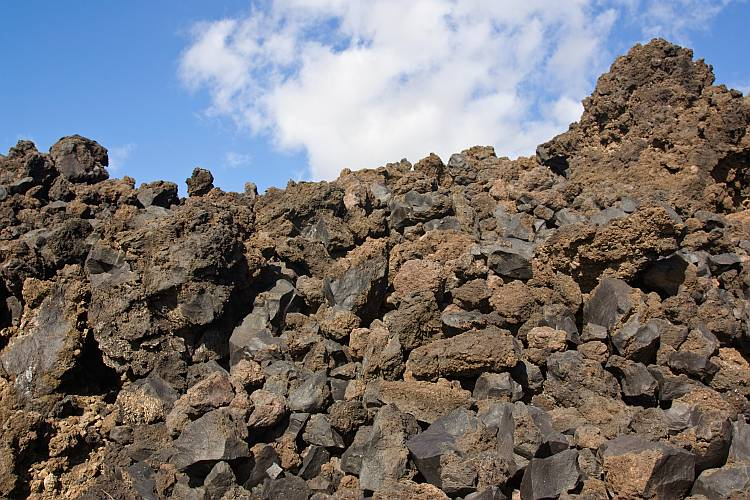
\includegraphics[width=\textwidth]{block_lava.jpg}$$

    \end{column}

  \end{columns}
  
\end{frame}
%-----------------------------------------------
\begin{frame}
  \frametitle{Lava domes}

  \begin{columns}[t]

    \begin{column}{0.48\paperwidth}

      Mound of viscous lava and rock around the vent \\

      \vspace{0.1cm}

      Can be crystal-poor or crystal-rich \\

      \vspace{0.1cm}

      Crystal-poor domes are rhyolitic \\

      \vspace{0.1cm}

      Crystal-rich domes span compositional spectrum \\

      \vspace{0.1cm}

      Common at convergent margins \\

      \vspace{0.1cm}

      Unstable collapse is a considerable hazard \\

      \vspace{0.1cm}

      Can grow \textbf{endogeneously} or \textbf{exogeneously} \\

      \vspace{0.1cm}

      Often associated with \textbf{vulcanian} explosions \\
    \end{column}

    \begin{column}{0.48\paperwidth}

      $$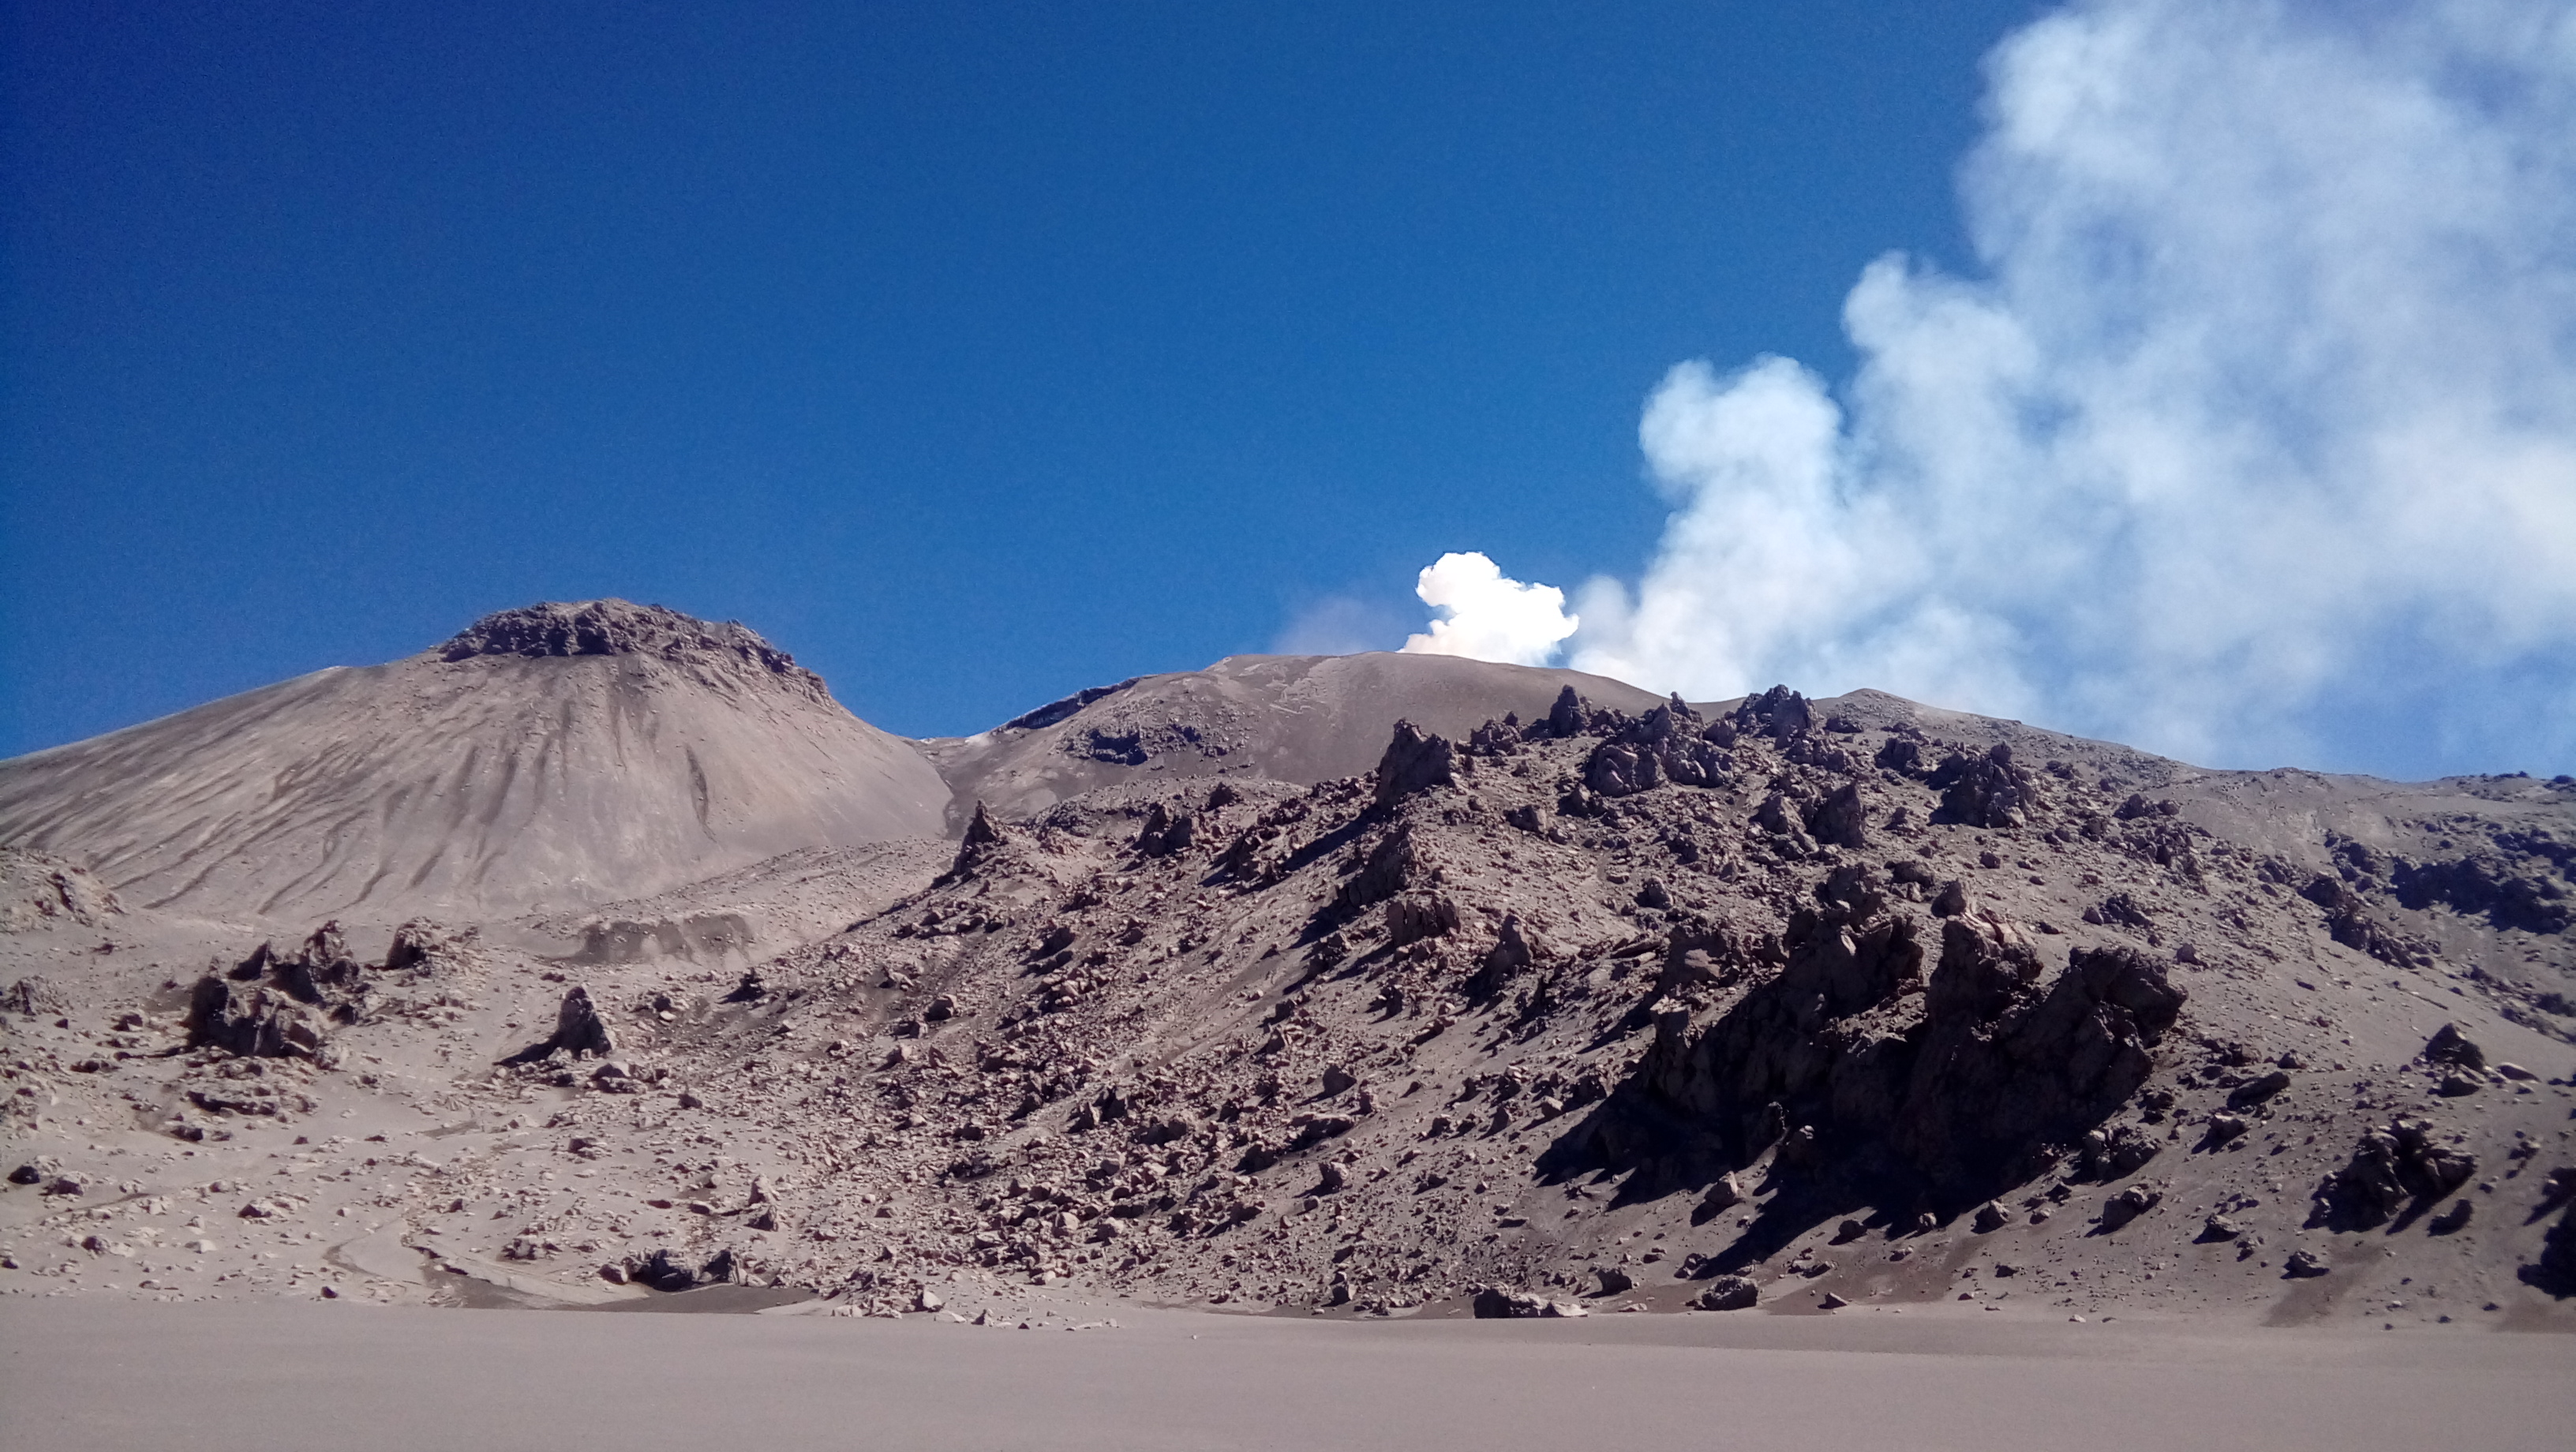
\includegraphics[width=\textwidth]{dome.jpg}$$

    \end{column}

  \end{columns}
  
\end{frame}
%-----------------------------------------------
\begin{frame}
  \frametitle{Spreading umbrella clouds}

  $$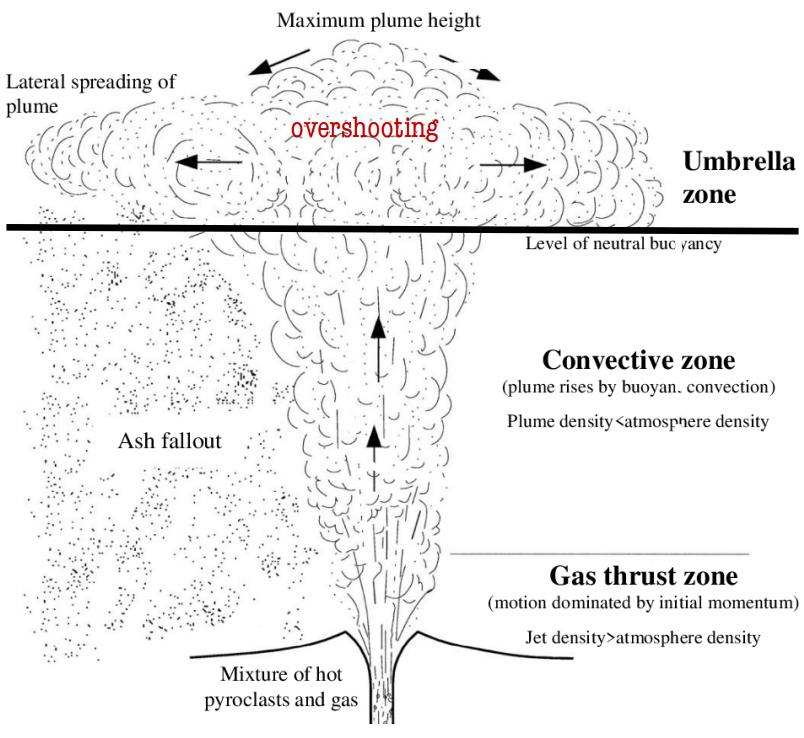
\includegraphics[width=0.7\textwidth]{plume.png}$$
  
\end{frame}
%-----------------------------------------------
\begin{frame}
  \frametitle{Spreading umbrella clouds}

  \begin{columns}[t]

    \begin{column}{0.5\paperwidth}

      \vspace{-1cm}
      
      $$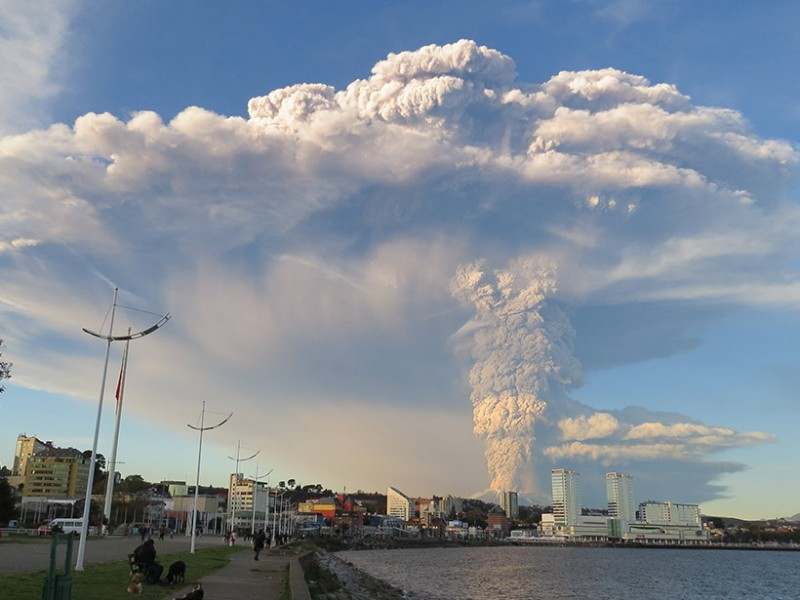
\includegraphics[width=0.95\textwidth]{calbuco.jpg}$$
      
      \vspace{-1cm}

      $$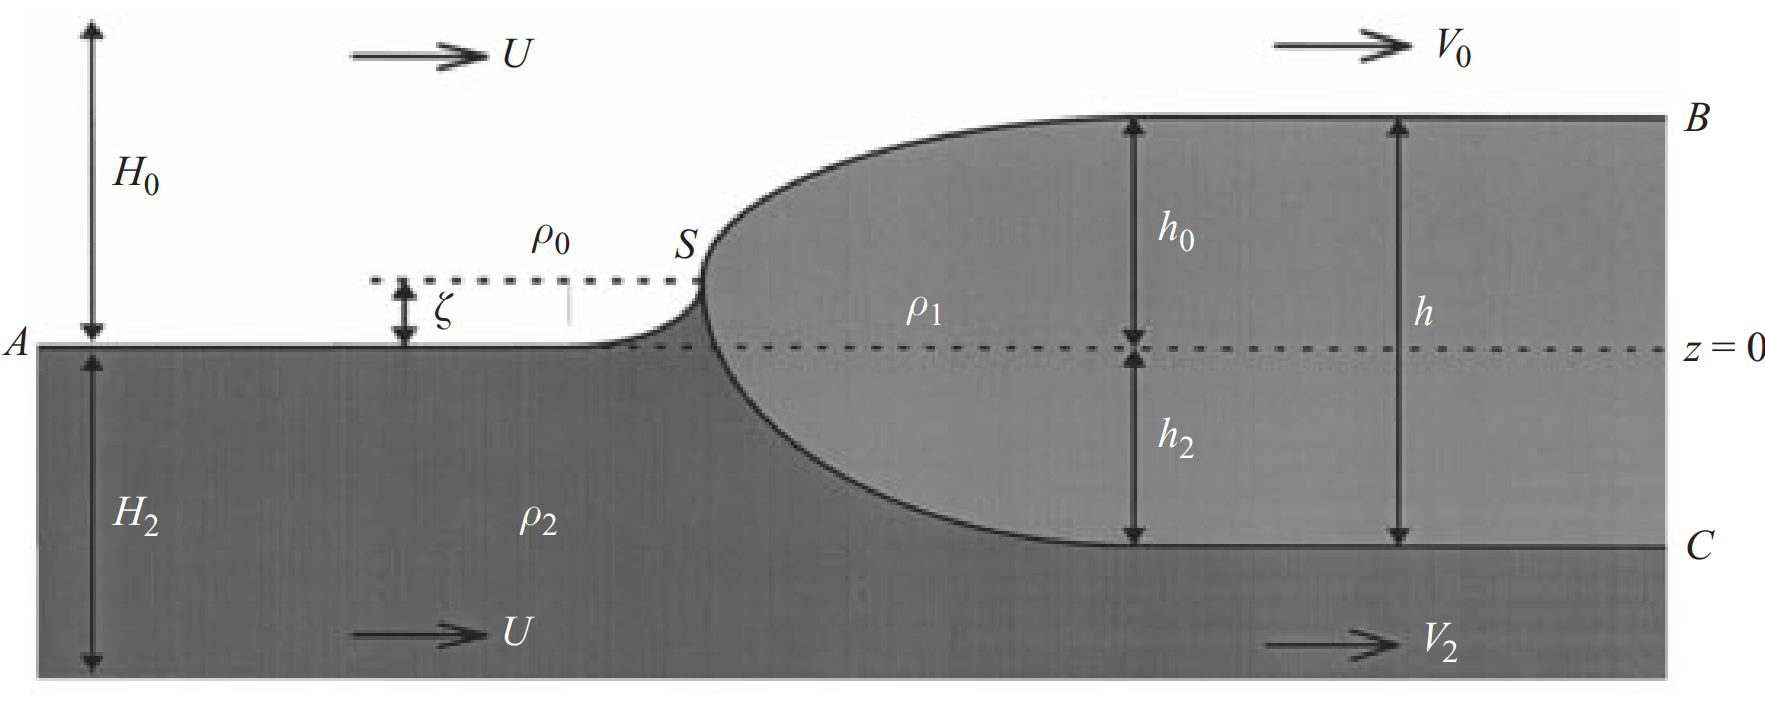
\includegraphics[width=0.95\textwidth]{interfacial_current.png}$$
      
    \end{column}

    \begin{column}{0.5\paperwidth}

      Radially spreading gravity current \\

      \vspace{-0.5cm}
      
      $$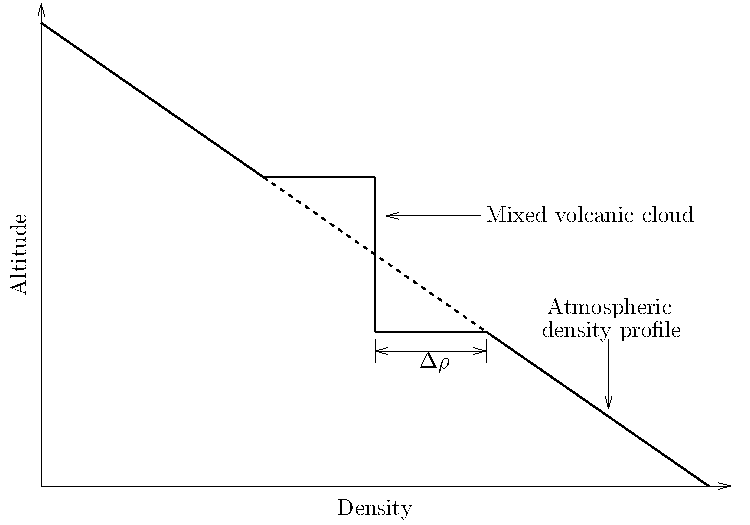
\includegraphics[width=0.95\textwidth]{dens_prof.pdf}$$

      Velocity depends on:

      \begin{itemize}
      \item Flux \\
      \item Density of mixture \\
      \end{itemize}
    \end{column}
    
  \end{columns}
  
\end{frame}
%-----------------------------------------------
\begin{frame}
  \frametitle{Spreading umbrella clouds: Experimental modelling}

  \movie{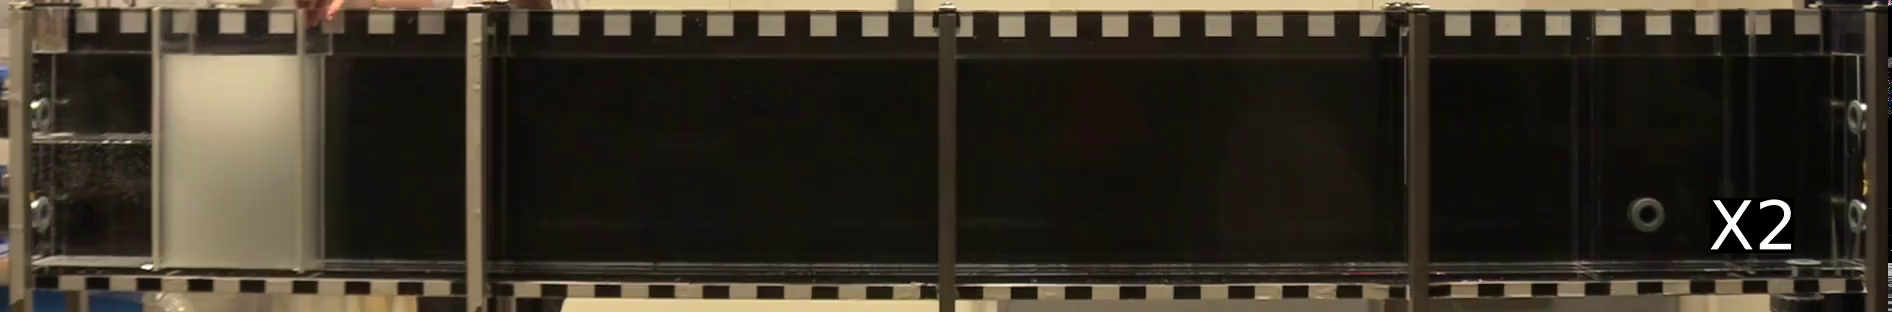
\includegraphics[width=\textwidth]{slow_x2.png}}{slow_x2.mp4}

  \movie{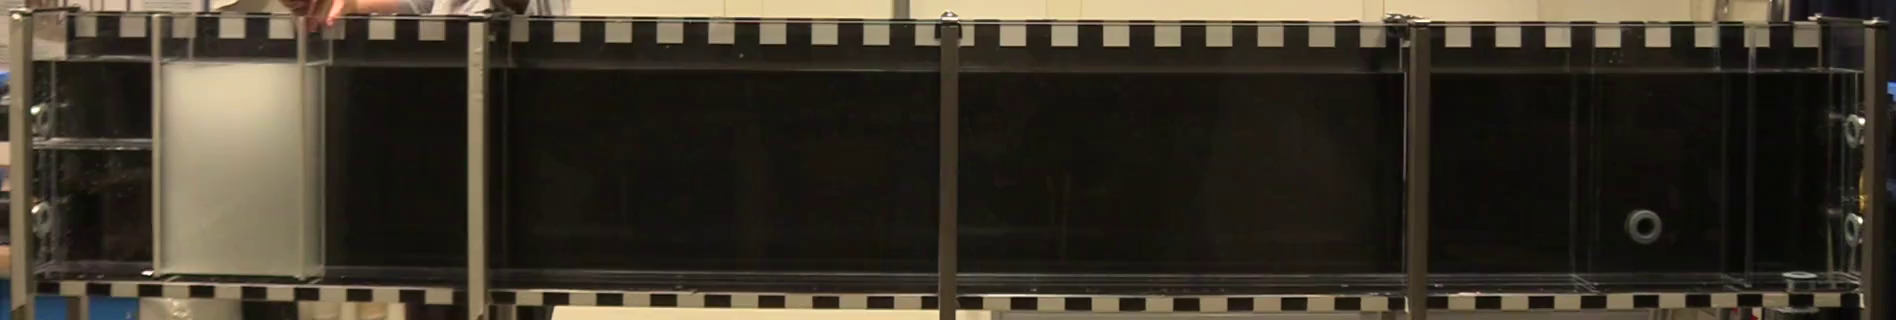
\includegraphics[width=\textwidth]{fast.png}}{fast.mp4}

  \vspace{0.5cm}
  
  Shear at the base of the cloud can inhibit fallout \\

  \vspace{0.5cm}
  
  Fallout can change density difference \\

  \vspace{0.5cm}
  
  Models of deposition from spreading clouds used to infer eruption parameters from deposit characteristics \\
  
\end{frame}
%-----------------------------------------------
\begin{frame}
  \frametitle{Pyroclastic density currents (PDCs): Generating mechanisms}

  \vspace{-0.7cm}
  
  \begin{columns}[t]

    \begin{column}{0.5\paperwidth}

      \vspace{-0.5cm}
      
      $$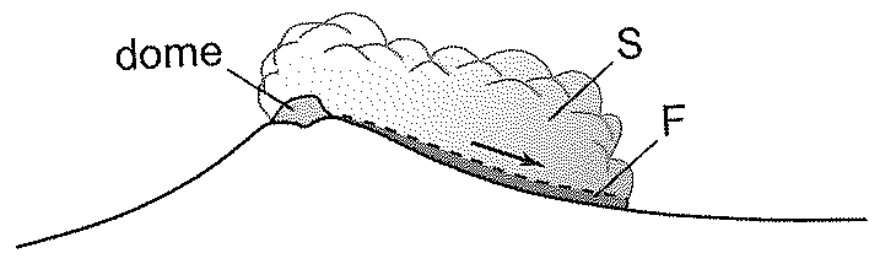
\includegraphics[width=0.8\textwidth]{dome_collapse.png}$$

      \vspace{-0.5cm}
      
      $$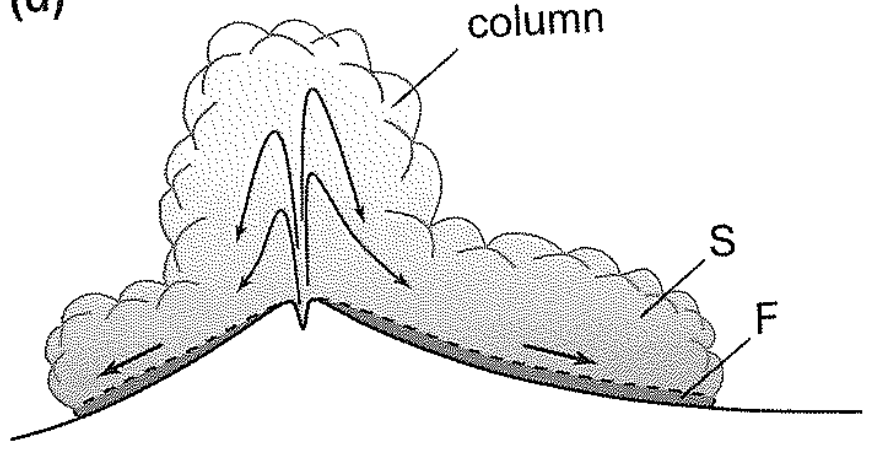
\includegraphics[width=0.8\textwidth]{column_collapse.png}$$

      \vspace{-0.7cm}
      
      $$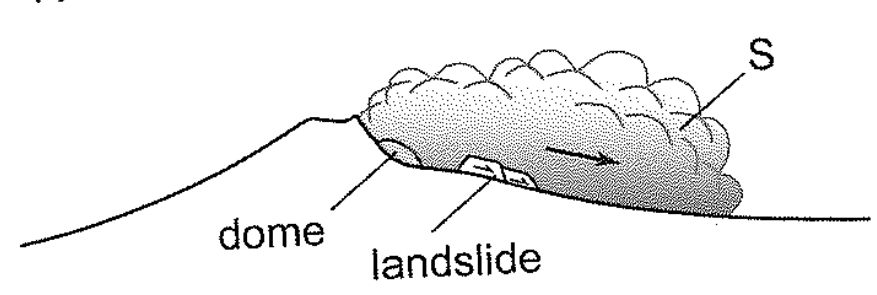
\includegraphics[width=0.8\textwidth]{lateral_blast.png}$$
    \end{column}

    \begin{column}{0.5\paperwidth}

      Dome collapse

      \begin{itemize}
      \item Front slope of dome becomes oversteep \\
      \item Material avalanches down slope \\
      \end{itemize}

      Column collapse

      \begin{itemize}
      \item Erupted jet doesn't become buoyant \\
      \item Material falls back to the ground  \\
      \end{itemize}

      Lateral blast

      \begin{itemize}
      \item Ground motion depressurises shallow magma \\
      \item Rapid expansion of volatiles mobilises more material  \\
      \end{itemize}
    \end{column}

  \end{columns}
  
\end{frame}
%-----------------------------------------------
\begin{frame}
  \frametitle{PDCs: Flows and surges}

  PDCs are a multiphase mixture of solid particles and hot gas \\

  \begin{columns}[t]

    \begin{column}{0.5\paperwidth}

      \small \textbf{Dilute surges}

      \begin{itemize}
      \item Solid concentrations $\sim$ 1 kg m$^{-3}$ \\
      \item Concentration increases downwards \\
      \item Velocity increases upwards \\
      \item Particle interactions negligible except at the base \\
      \end{itemize}

      \textbf{Dense flows}

      \begin{itemize}
      \item Particle concentrations similar to that in the deposit \\
      \item Internal velocity and concentration profiles poorly constrained \\
      \end{itemize}
    \end{column}

    \begin{column}{0.5\paperwidth}

      $$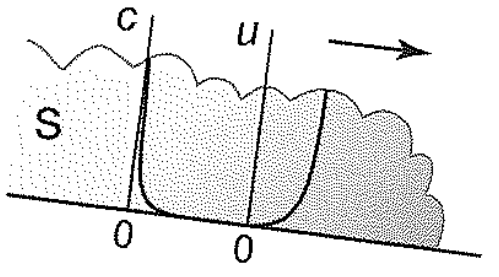
\includegraphics[width=0.8\textwidth]{dilute_PDC.png}$$

      \vspace{-0.5cm}
      
      $$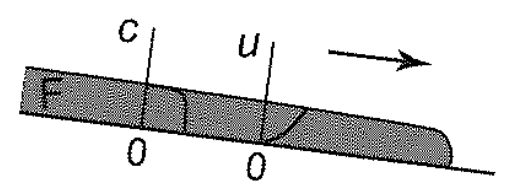
\includegraphics[width=0.8\textwidth]{dense_PDC.png}$$
      
    \end{column}

  \end{columns}
  
\end{frame}

%-----------------------------------------------
\begin{frame}
  \frametitle{Surges: Effect of particle sedimentation and mixing}

  \movie{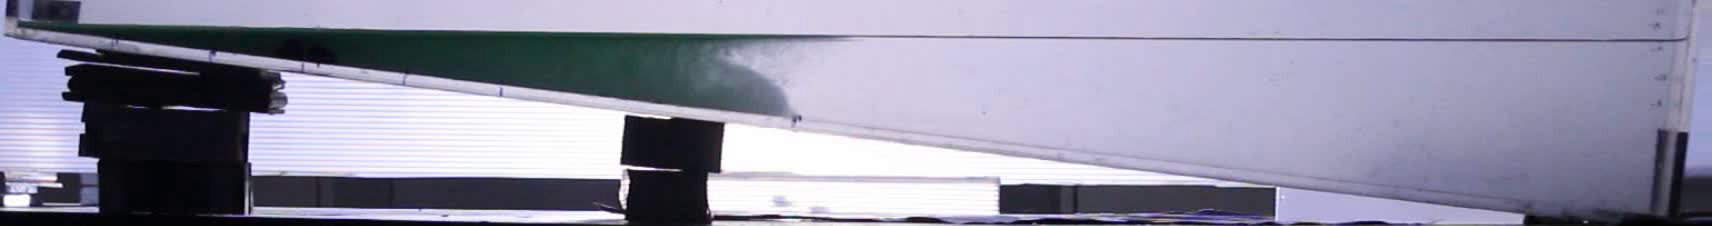
\includegraphics[width=\textwidth]{Sutherland18.png}}{Sutherland18.mp4}
  \begin{center}
    \footnotesize Sutherland et al. (2018)
  \end{center}

  To model current propagation need to consider conservation of:

  \begin{itemize}
  \item Mass \\
  \item Momentum \\
  \item Energy \\
  \end{itemize}

  How do particle settling and mixing affect these balances? \\
\end{frame}
%-----------------------------------------------
\begin{frame}
  \frametitle{Flows: Detailed study on internal structure}

  \movie{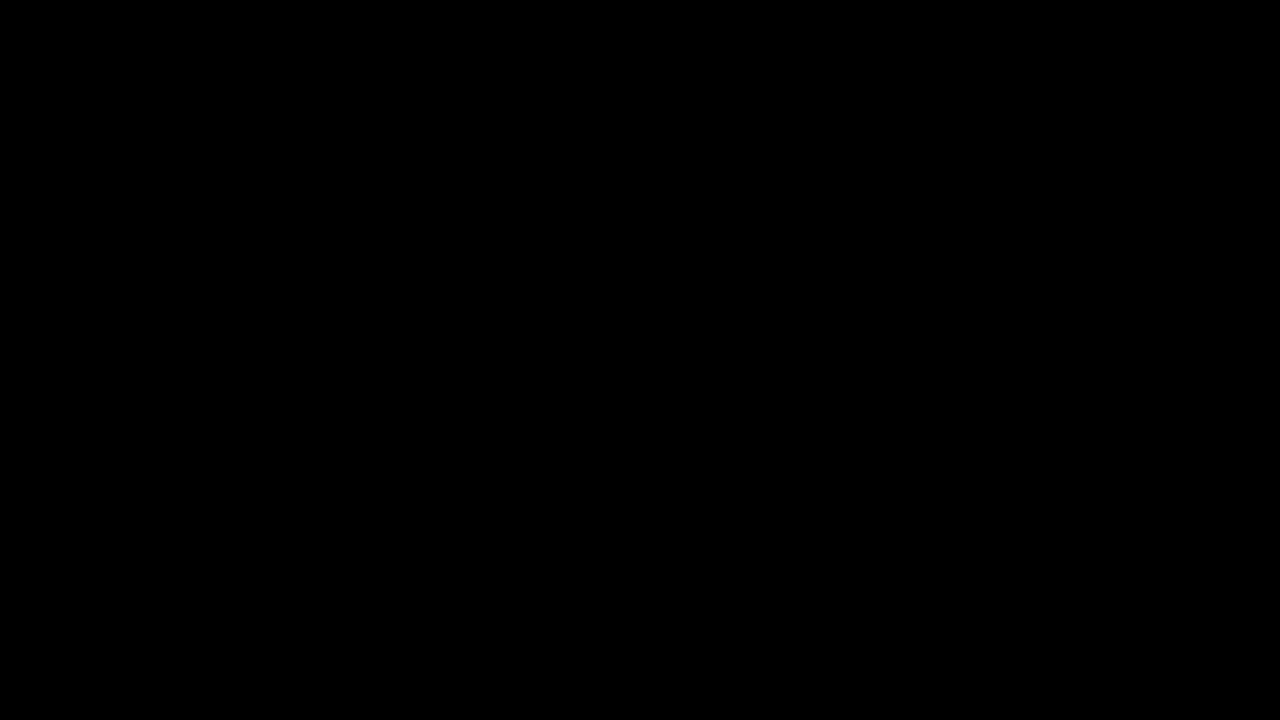
\includegraphics[width=\textwidth]{Lube19_1.png}}{Lube19_1.mp4}
  \begin{center}
    \footnotesize Lube et al. (2019)
  \end{center}

\end{frame}
%-----------------------------------------------
\begin{frame}
  \frametitle{Flows: Detailed study on internal structure}

  \movie{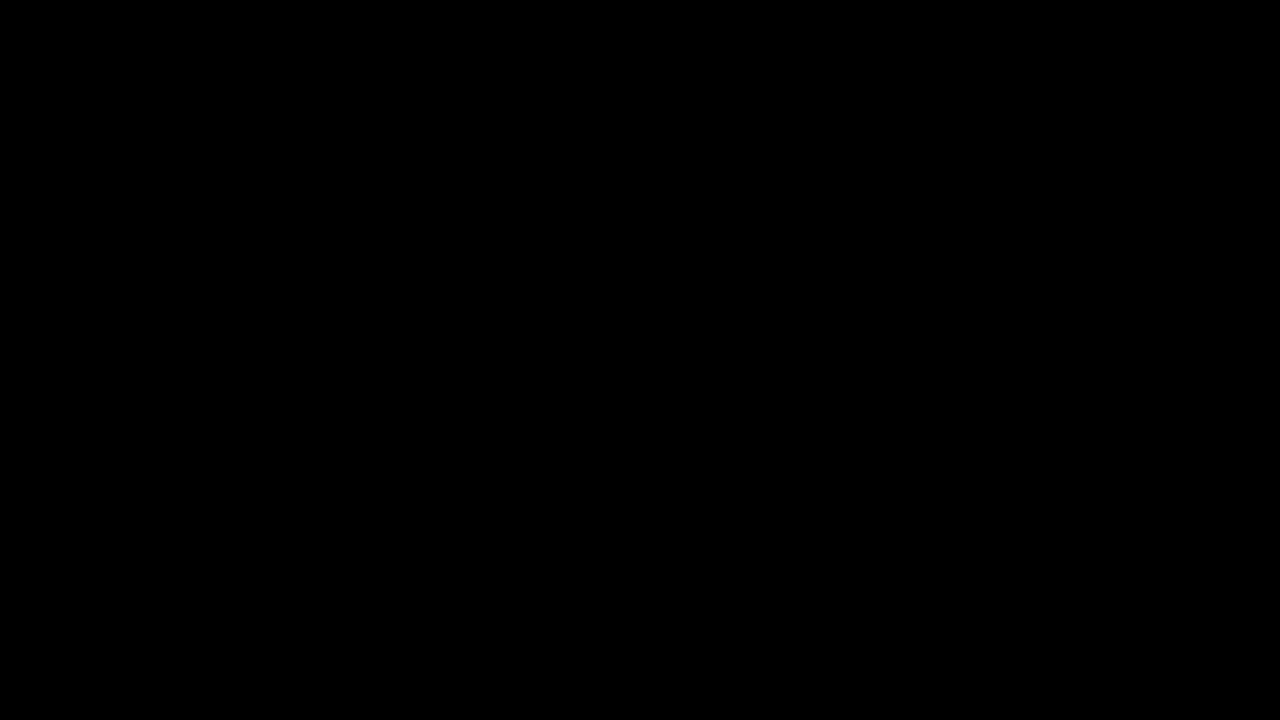
\includegraphics[width=\textwidth]{Lube19_2.png}}{Lube19_2.mp4}
  \begin{center}
    \footnotesize Lube et al. (2019)
  \end{center}

\end{frame}
%-----------------------------------------------
\begin{frame}
  \frametitle{Lahars: Remobilised pyroclastic deposits}

  \textbf{Lahars} - Mixtures of water and volcaniclastic sediment \\

  \begin{columns}[t]

    \begin{column}{0.48\paperwidth}

      Huge variation in:

      \begin{itemize}
      \item Volume: $10^{2} - 10^{9}$ m$^{3}$ \\
      \item Peak discharge: $<10 - 10^{7}$ m$^{3}$ s$^{-1}$ \\
      \item Advance rate: $\sim 2 - 80$ m s$^{-1}$ \\
      \item Runout: $<10 - >100$ km \\
      \end{itemize}

    \end{column}

    \begin{column}{0.48\paperwidth}

      $$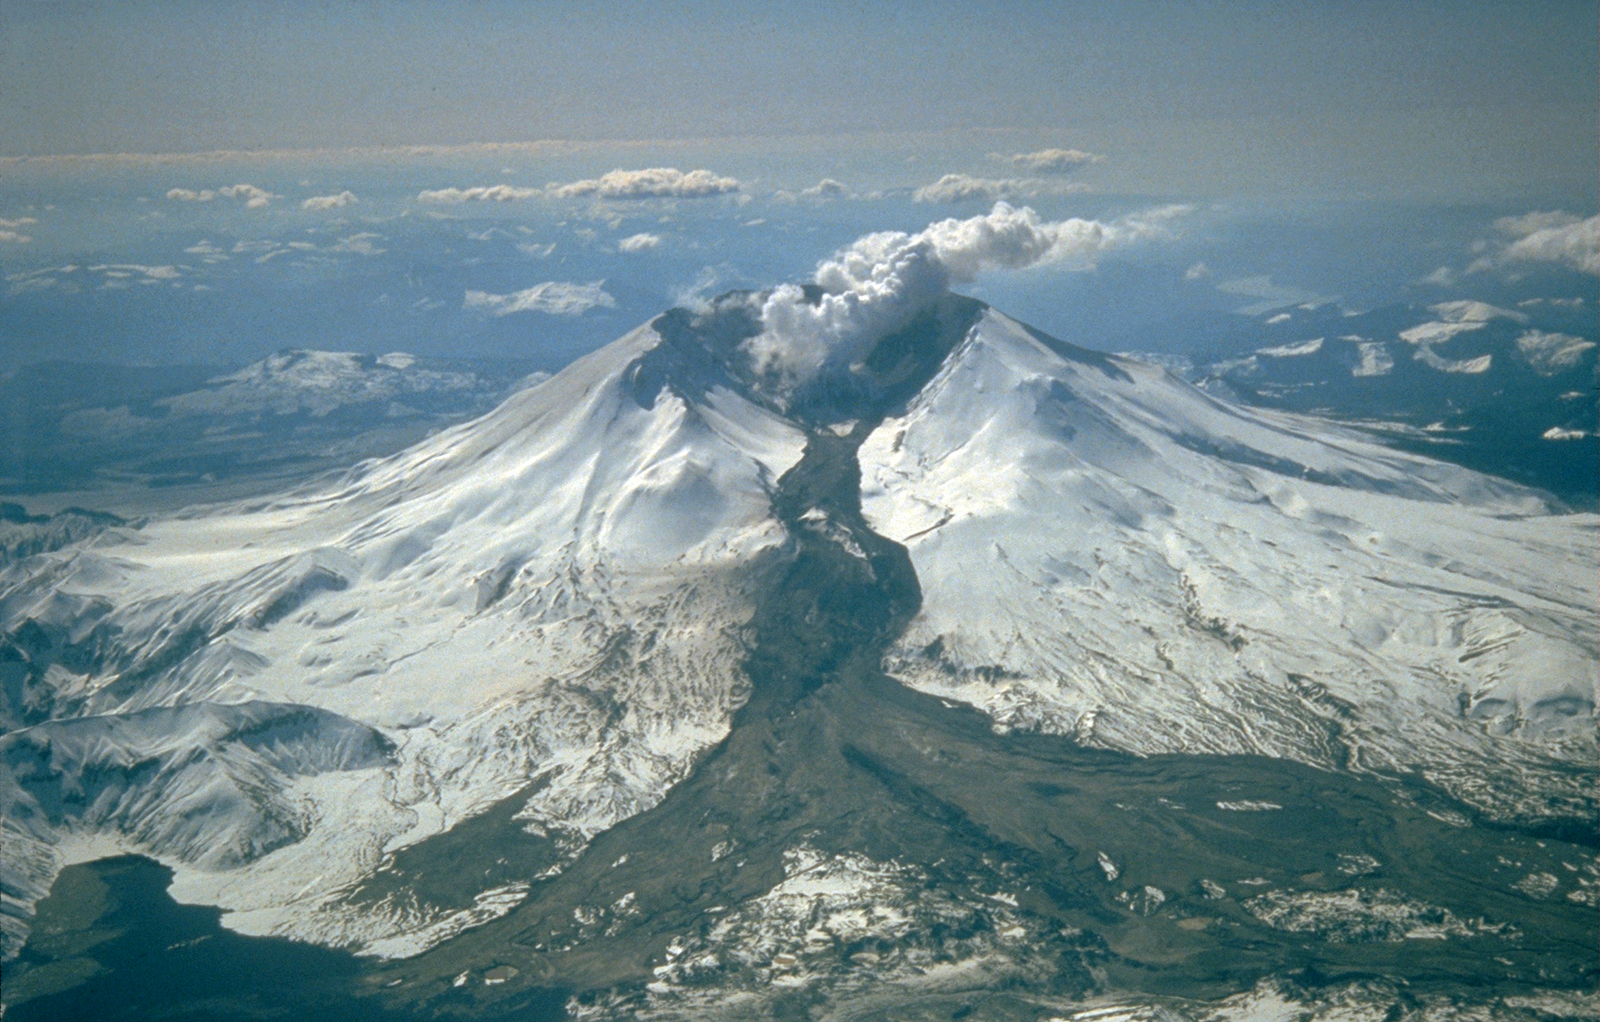
\includegraphics[width=\textwidth]{msh_lahar.jpg}$$

    \end{column}

  \end{columns}
  
\end{frame}
%-----------------------------------------------
\begin{frame}
  \frametitle{Lahar triggering}

  \begin{columns}[t]

    \begin{column}{0.48\paperwidth}
      
      Lahar initiation requires:

      \begin{itemize}
      \item Sufficient water supply \\
      \item Adundant unconsolidated sediment \\
      \item Gravitational potential \\
      \item Triggering mechanism \\
        \begin{itemize}
        \item Rainfall \\
        \item Snow and ice melt \\
        \item Liquefaction \\
        \end{itemize}
      \end{itemize}

    \end{column}

    \begin{column}{0.48\paperwidth}

      $$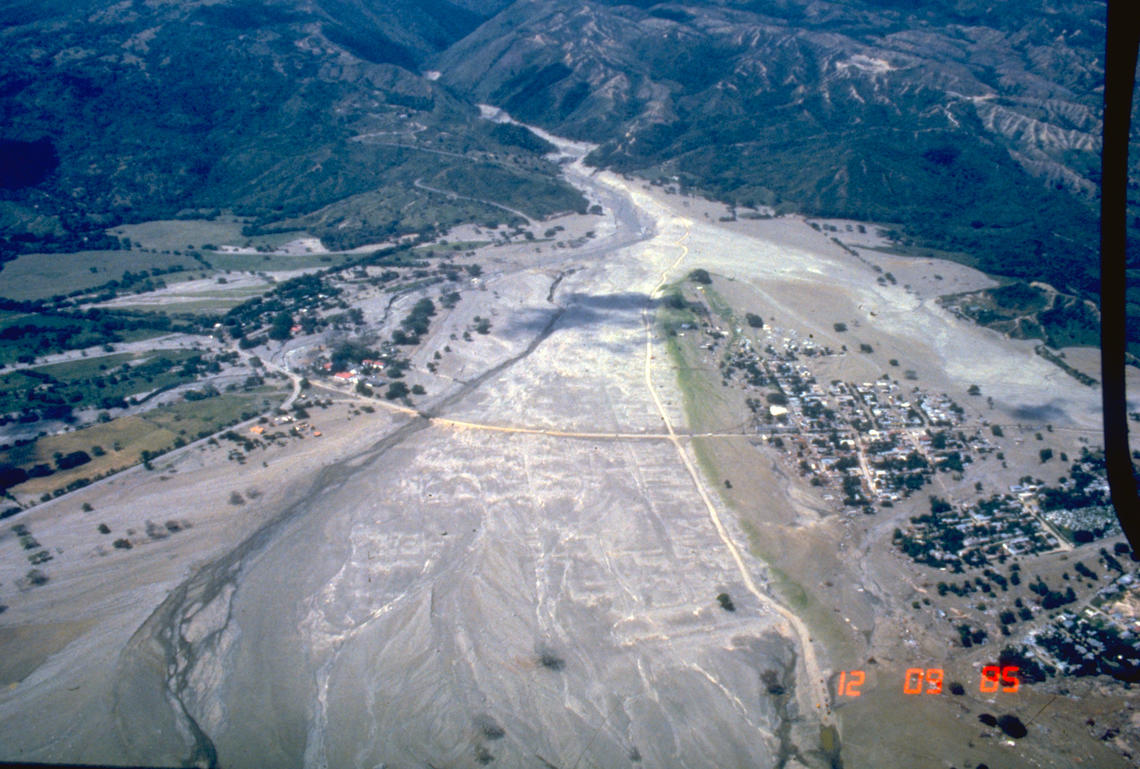
\includegraphics[width=\textwidth]{ndr_lahar.jpg}$$

    \end{column}

  \end{columns}
    
\end{frame}
%-----------------------------------------------
\begin{frame}
  \frametitle{Lahar rheology}

  \begin{columns}[t]

    \begin{column}{0.48\paperwidth}
      
      \textbf{Hyperconcentrated flow}

      \begin{itemize}
        \item Solid volume fraction $\sim$ 0.2-0.5 \\
        \item Bulk density $\sim$ 1.3-1.8 kg m$^{-3}$ \\
        \item Density stratified \\
        \item Turbulent \\
      \end{itemize}

      \textbf{Debris flow}

      \begin{itemize}
      \item Solid volume fraction $\sim$ 0.5-0.8 \\
      \item Bulk density $\sim$ 1.8-2.3 kg m$^{-3}$ \\
      \item $10^{4}$ - 10$^{5}$ times more viscous than water \\
      \end{itemize}
      
    \end{column}

    \begin{column}{0.48\paperwidth}

      $$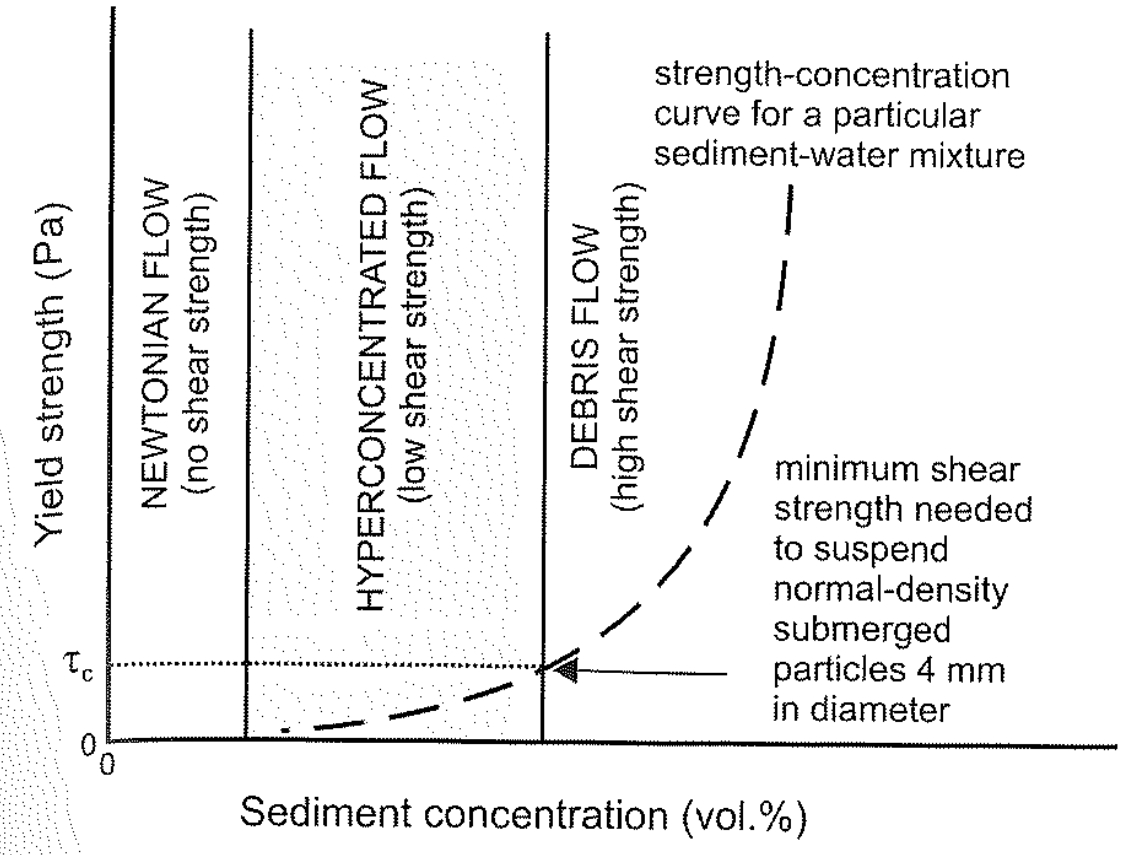
\includegraphics[width=\textwidth]{lahar_rheo.png}$$

    \end{column}

  \end{columns}
    
\end{frame}
%-----------------------------------------------
\begin{frame}
  \frametitle{Conclusions}

  \begin{itemize}
  \item Volcanoes are sources for various gravity currents \\
  \item Reynolds number $\text{Re}$ strongly determines style of flow \\
  \item Lava flows have low $\text{Re}$ \\
  \item Volcanic clouds, PDCs and lahars have high $\text{Re}$ \\
  \item Multiphase nature of flows exerts strong control on flow runout and deposit morphology \\
  \item Hazard and risk assessment requires these flows to be modelled \\
  \end{itemize}

    
\end{frame}
%-----------------------------------------------



\end{document}
